%
% A New Frontier - Towards the Singularity
%

\section{A new frontier -- Towards the singularity} \label{sec:outlook} \index{Outlook} \index{A new frontier}

In this section we provide a non-technical outlook on the future quantum internet and its implications, for the benefit of the technically disinterested reader. This section is in the form of several short essays, requiring no technical background knowledge in quantum computation, quantum mechanics, or mathematics.

We acknowledge that while parts of these essays are highly plausible, if not certain, others are highly speculative, but nonetheless based on believable although somewhat futuristic reasoning. At the very least we hope to stimulate the exchange of ideas and their development. We encourage the reader to question the ideas presented in these essays and put forth their own ideas and predictions.

\textit{``There is no harm in doubt and skepticism, for it is through these that new discoveries are made.''} --- Richard Feynman.

%
% The Era of Quantum Supremacy
%

\section{The era of quantum supremacy} \label{sec:era_quant} \index{Quantum supremacy}

\dropcap{A}{} pertinent question to ask is `What is the timescale for useful quantum technologies? When will they be viable?'. The correct answer is likely very soon.

From the perspective of classical computing, Moore's Law (observation!)\index{Moore's Law} for the exponential growth trend in classical computing power has proven to be a very accurate one. In Fig.~\ref{fig:moores_law} we illustrate the historical evolution in classical computing power, and extrapolate 5 years into the future.\index{Moore's Law}

\begin{figure}[!htb]
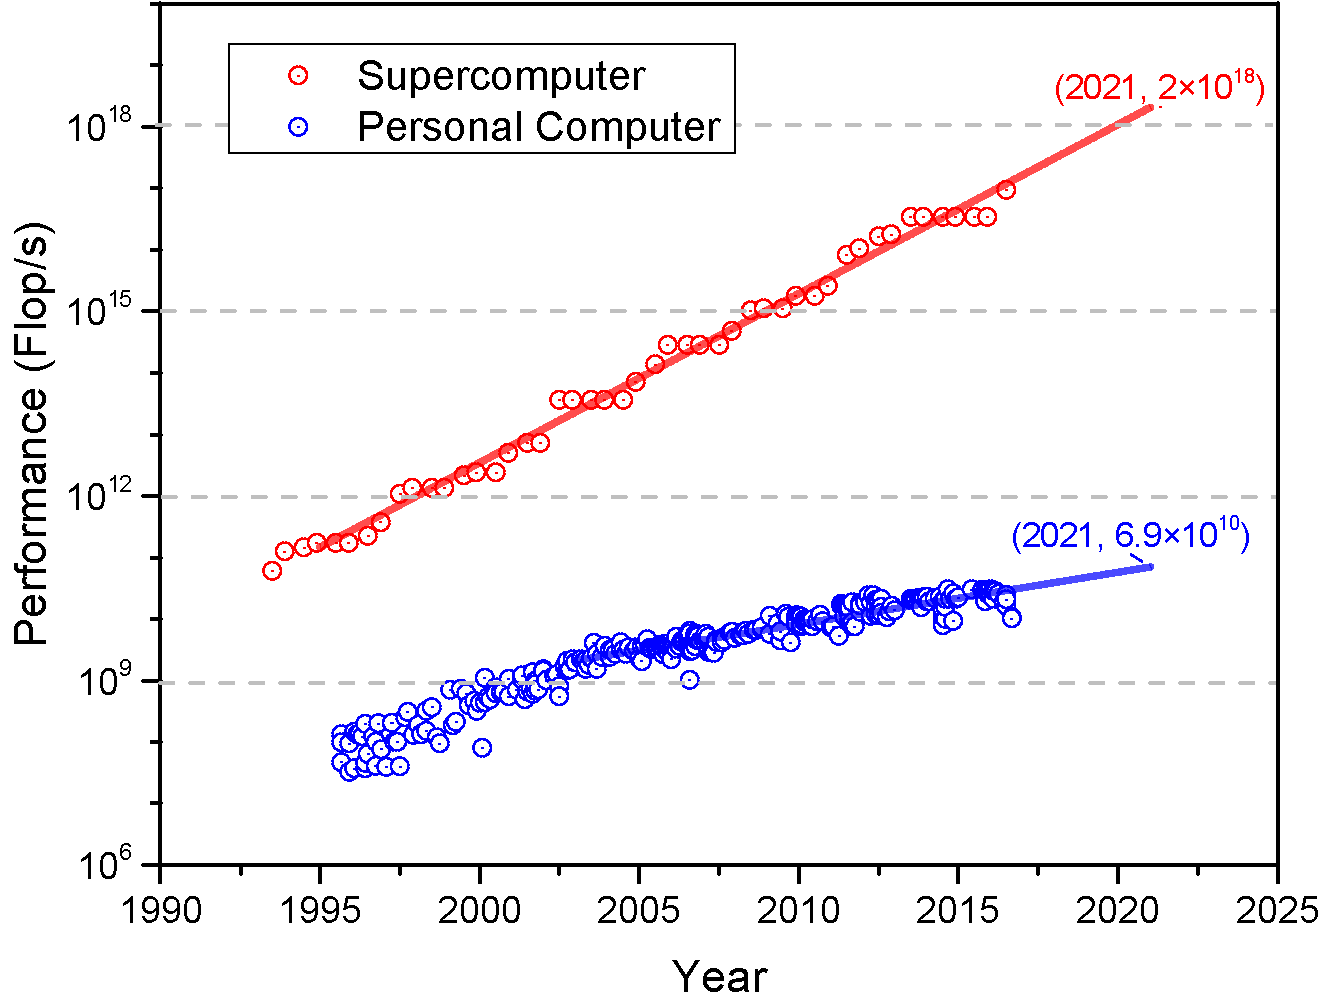
\includegraphics[width=0.47\textwidth]{moores_law}
\caption{Historical trends in classical computing power for both PCs and top-end supercomputers, with an extrapolation 5 years into the future. The close fit to exponential growth in performance over time is apparent from the logarithmic scale.} \label{fig:moores_law}
\end{figure}

To put this into context, current day microprocessors contains on the order of billions of single transistors. Current day  experimental quantum computers, on the other hand, contain fewer than 100 qubits. We sit at the mere very beginning of Moore's adventure through the quantum era.

%As a comparison we compare this to the \textsc{BosonSampling} \comment{NO BOSON-SAMPLING. MAKE SUPERIMPOSED PLOT COMPRISING ALL ARCHITECTURES AND DEVELOPMENTS. TRY TO EXTRAPOLATE} (Sec.~\ref{sec:BS})\index{Boson-sampling} model for restricted quantum computation, as it is perhaps the most plausible candidate for the first demonstration of quantum computational supremacy. The relationship between \textsc{BosonSampling} photon-number and classical equivalent processing power is shown in Fig.~\ref{fig:moores_super}.

%\begin{figure}[!htb]
%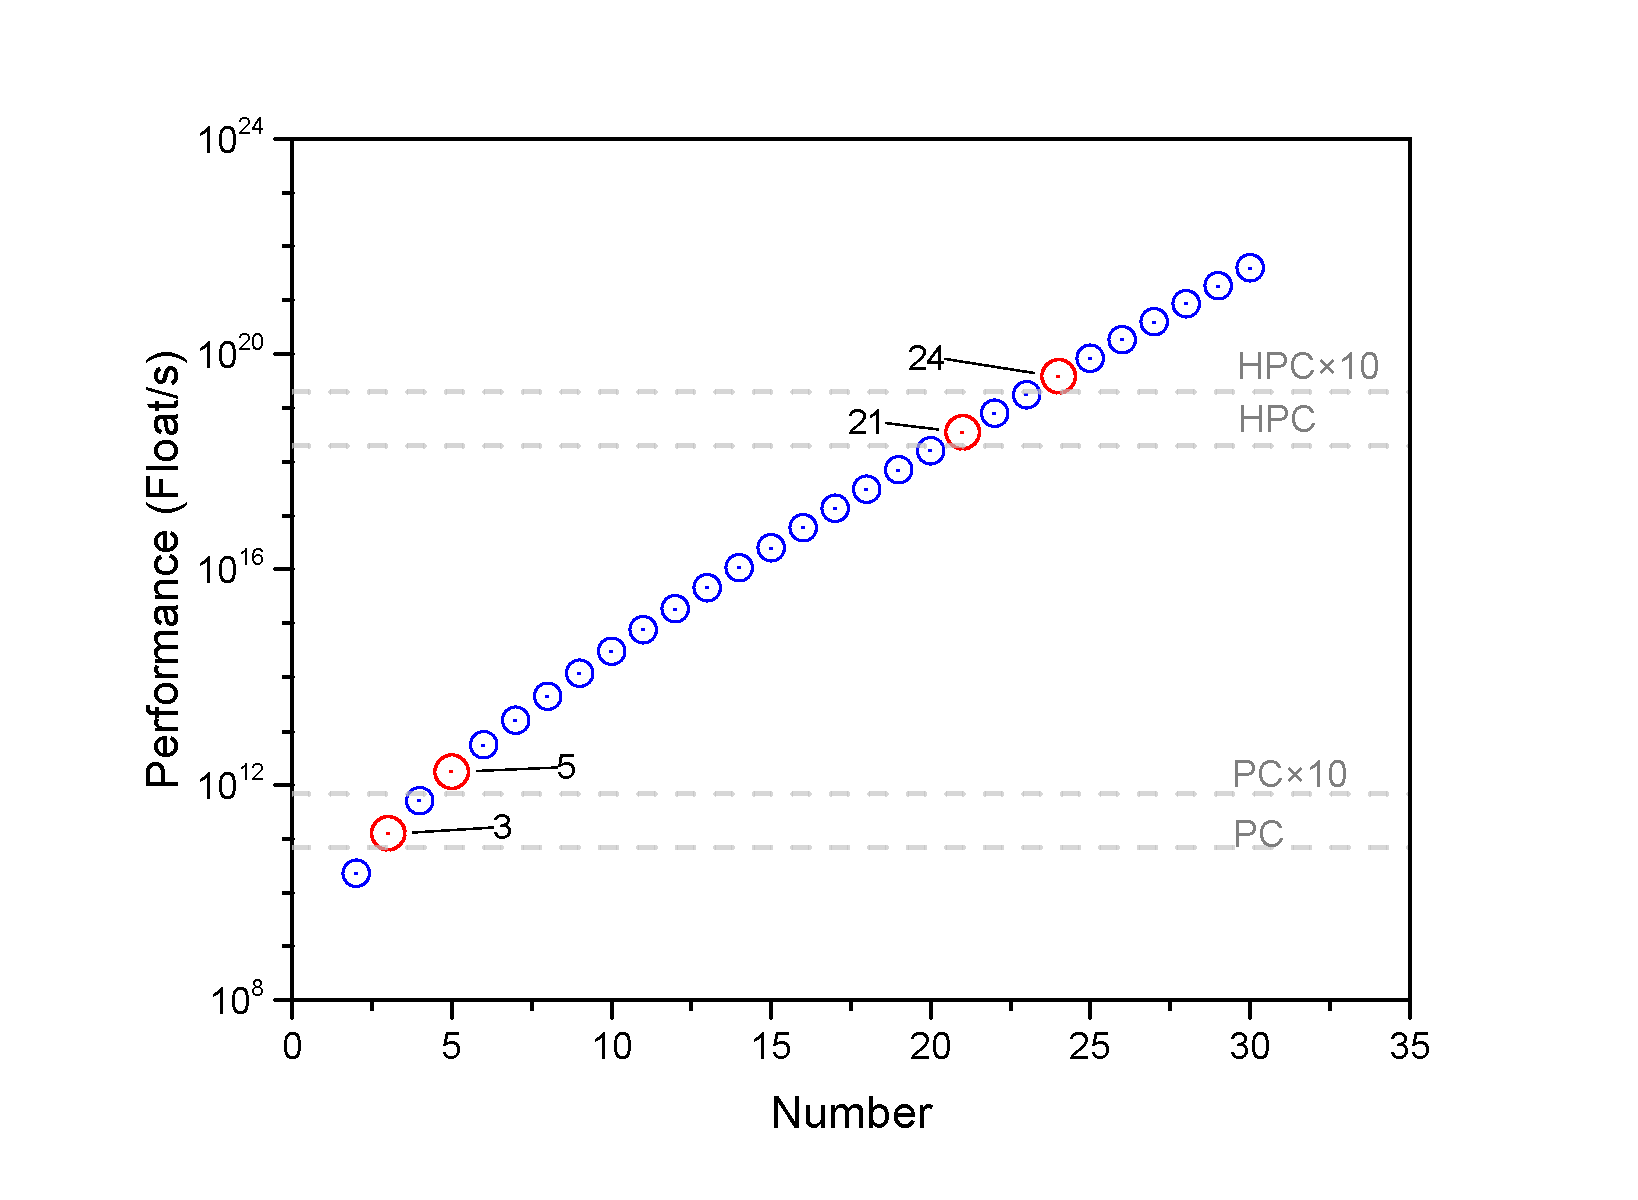
\includegraphics[width=0.47\textwidth]{moores_super}
%\caption{Relationship between photon-number and classical equivalent FLOPS for `scattershot' \textsc{BosonSampling}. The annotated red data-points show several points of interest, taking a Moore's Law extrapolation of classical computing power 5 years into the future for desktop PCs and top-end high-performance computers, as well as an order of magnitude greater performance respectively. We use these as indicators of the post-classical era.} \label{fig:moores_super}
%\end{figure}

%\comment{Based on these extrapolations}, \cite{CYLu} \comment{(Need to revise the numbers, cite Montanaro et al. on classical simulation of boson-sampling)} \comment{made the prediction that a \textsc{BosonSampling} computer could outperform top-end supercomputers of 5 years into the future by an order of magnitude (a fairly reasonable benchmark for usage of the term `post-classical') using just \mbox{$\sim 24$} photons. Given that present-day experimental efforts have recently reached 10 photons \cite{bib:tenPhotEnt}, with great ambitions to scale up further, it is to be expected that the post-classical era is imminent. Whilst it is difficult to predict exactly when technology will allow a bank of 24 high-fidelity, highly-indistinguishable, push-button (or heralded) single-photon sources operating in parallel, it seems fair to predict that the timescale will be on the order of years rather than decades.}

%\comment{However, be weary that we are being a little optimistic with this statement, since \textsc{BosonSampling} is not universal for quantum computation, and doesn't even have any known practical uses, i.e it's post-classical and that's about it! It would be more helpful to consider prospects for \textit{universal} quantum computation.}

While the power of classical computers scales at most linearly with the number of transistors, the classical-equivalent power\index{Classical-equivalent computational power} of quantum computers scales exponentially with the number of qubits (in the best-case scenario). The classical Moore's Law is close to saturation -- we simply can't make transistors too much smaller than they already are\footnote{Current transistor feature sizes are on the order of several hundred atoms. Under a Moore's Law prediction, we are likely to hit fundamental physical barriers in transistor size within a decade. We can't make a transistor smaller than an atom!}! We therefore envisage a new Quantum Moore's Law, which follows a far more impressive trajectory than its classical counterpart. The point of critical mass in quantum computing will take place when the classical and Quantum Moore's Law extrapolations intersect, signalling the commencement of the \textit{post-classical era}\index{Post-classical era}. Estimating this is more challenging than it sounds, since although the classical Moore's Law is extremely well established with an excellent fit to an exponential trajectory, there aren't yet enough data-points to make a confident prediction about a Quantum Moore's Law, to what trajectory it best fits, and at what rate it progresses.

Aside from quantum computing, theoretically unbreakable quantum crypto-systems, in the form of quantum key distribution (QKD), are already technologically viable\index{Quantum key distribution (QKD)}, and are in fact commercially available off-the-shelf today, as end-to-end units connectable via fibre-optics. Recently, satellite-based QKD was demonstrated, enabling direct intercontinental QKD over thousands of kilometres. Although only a single such satellite has been demonstrated, its success implies that constellations of interconnected such satellites are inevitable in the near future, enabling point-to-point QKD between any two points on Earth. It is likely the next space-race will be the one for quantum supremacy.

As the era of post-classical quantum computation edges closer, the importance of QKD networks will intensify, and along with it the demand for quantum networking infrastructure.

It is clear that humanity already sits at the precipice of harnessing quantum technologies, and must act quickly to enable them to be fully exploited as they emerge in the near future.

%
% The Economics of the Quantum Internet
%

\subsection{The economics of the quantum internet} \label{sec:economics} \index{Economics}

Quantum computers are highly likely to, at least initially, be extremely expensive, and affordable outright by few. Thus, client/server economic models based on outsourcing of computations to servers on a network, will be essential to making quantum computing widely accessible. The protocols we have presented here pave the way for this type of economic model to emerge. It is paramount that the types of technologies introduced here be fully developed in time for the deployment of useful quantum computing hardware, such that they can be fully commercialised from day one of their availability, enabling widespread adoption, enhanced economy of scale, and rapid proliferation.

A key question regarding the economics of the quantum internet is the extent to which it will be able to piggyback off existing optical communications infrastructure, given that networking will almost inevitably be optically mediated. We have an existing intercontinental fibre-optic backbone, as well as sophisticated satellite networks. To what extent will this existing infrastructure (or future telecom/satellite infrastructure) be able to be exploited so as to avoid having to rebuild the entire future quantum internet infrastructure from scratch? This is a question worth billions of dollars. We also need to factor in that given the massive driving force behind telecom technology, its cost is following a Moore's Law-like trajectory of its own, and what costs a billion dollars today might cost a million dollars in a decade's time. In light of this, telecom wavelength quantum optics is being hotly pursued. And at the time of writing this paragraph, a world-leading Chinese experimental team has just successfully launched a QKD satellite into low Earth orbit \cite{???}, enabling intercontinental entanglement distribution and QKD, with talk of the next space race being the one for quantum supremacy \cite{???}.

Technology should benefit humanity, not only an elite few --- \textit{Homo sum humani a me nihil alienum puto}. In light of this, who exactly will benefit from the quantum internet? Its beauty is that it doesn't create a system of winners and losers. Rather, it establishes a technological infrastructure from which all can benefit, rich or poor. Well-resourced operators who can afford quantum computers, for example, will benefit from being able to license out compute time on their computers, ensuring no wasted clock-cycles and maximising efficiency. The less-well-resourced will benefit in that they will have a means by which to access the extraordinary power of quantum computing on a licensed basis, facilitating access to infrastructure by those who otherwise would have been priced out of the market. This is essentially the same model as what is employed by some present-day supercomputer operators, enabling small players access to supercomputing infrastructure. The quantum internet is critical to achieving the same goal in the quantum era. This could have transformative effects on the developing world in particular. And many emerging industries, for whom access to quantum computation will be critical, but who cannot afford them, will benefit immensely from the client/server model.

Already today, even before the advent of useful post-classical quantum computers, we are seeing the emergence of the outsourced model for computation\index{Outsourced quantum computation}. IBM recently made an elementary 16-qubit quantum computer freely available for use via the cloud. Interested users can log in online, upload a circuit description for a quantum protocol, and have it executed remotely, with the results relayed back in real-time. Although still very primitive, this simple development already makes experimentation with elementary quantum protocols accessible to the poor layman, undergrad, or PhD student in a developing country, people who just last year would never have dreamt of being able to run their own quantum information processing experiments! This effectively opens up research opportunities to people who otherwise would have been priced out of the market entirely, unable to compete with established, well-resourced labs. Evidently, the market already recognises the importance of outsourced models for quantum computation. We encourage the impatiently curious reader to log onto the `IBM Quantum Experience' (\texttt{\href{http://www.research.ibm.com/quantum/}{http://www.research.ibm.com/quantum/}}) and take a shot at designing a 16-qubit quantum protocol, without even needing to be in the same country as the quantum computer.

The quantum internet will facilitate the communication and trade of quantum assets beyond just quantum computation and cryptography. There are many uses for various hard-to-prepare quantum states, for example in metrology, lithography, or research, where outsourcing complicated state preparation would be valuable. Alternately, performing some quantum measurements can be technologically challenging, and the ability to delegate them to someone better-equipped would be desirable. The quantum internet goes beyond just quantum computing. Rather, it extends to a full range of quantum resources and protocols.\index{State preparation} \index{Measurement}

To commodify quantum computing, if constructing large-scale quantum computers were a simple matter of plug-and-play, where QuantumLego\texttrademark \,building blocks are available off-the-shelf and straightforward to assemble even for monkeys, mass production would rapidly force down prices. By arbitrarily interconnecting these boxes, large-scale quantum computers could be scaled up with demand, with a trajectory following a new Quantum Moore's Law, with potentially super-exponential computational return.

We envisage that each of these commodity items is a black box, within which a relatively small number of qubits are held captive. Then, to build a larger quantum computer, we don't need to upgrade our boxes. Rather, we simply purchase more boxes to interconnect over the network. This notion is tailored to cluster states in particular -- because a cluster state can be realised by nearest neighbour interactions alone, and since all preparation stages commute with one another, they naturally lend themselves to modularised, distributed preparation.\index{Modularised quantum computation}

Such an approach lends itself naturally to distributed computation, where modules may be shared across multiple users, with the economic benefit of maximising resource utilisation, and the practical benefit of the end-user effectively having a much larger quantum computer at their disposal.\index{Distributed quantum computation}

By having a standardised architecture for optically interconnecting modules, we also somewhat `future-proof' our hardware investment -- if interfacing modules is standardised, existing hardware can be fully compatible with newer, more capable module versions. We might envision the emergence of open standards on optical interconnects and fusion protocols.

On the other hand, if quantum computers were only ever sold as specialised, room-sized, all-in-one solutions (think D-Wave\texttrademark), such mass production would not experience the driving force of commodified, off-the-shelf building blocks, each of which is cheap, yet frugal in its computational power alone.

Essential to existing financial markets are pricing models for physical assets. Furthermore, derivative markets increase trading liquidity, market efficiency, enhance price discovery, and importantly, allow risk management via hedging and the ability to lock in future prices. This is invaluable to traders of conventional commodities, and it is to be expected that it will be equally valuable to consumers of quantum resources. We have made initial steps in deriving pricing models for quantum assets and derivatives, which although they may require revision in the future real-world quantum marketplace, provide an initial qualitative understanding of quantum market dynamics. \comment{Advantages of derivatives}

Networked quantum computing will present new challenges for policy-makers, whose fiscal policies strive to maximise economic efficiency and optimise resource allocation. Devising policies of taxation and a regulatory framework in the quantum era will require careful deliberation.

It is evident that taxation of qubits has far deeper economic implications than the taxation of other typical financial assets or classical technologies, owing to their exponential scaling characteristics. Generally speaking, taxation of an asset disincentivises its growth. But if the computational return on quantum assets grows exponentially with network size, so too will sensitivity to taxes that stifle it. This will require extremely prudent consideration when designing tax policies in the quantum era, so as to avoid exponential suppression of quantum-related economic activity.

Conversely, the exponential dependence on the rate of taxation could be exploited for leverage via subsidisation. It may be economically beneficial to subsidise quantum infrastructure, reaping its exponential payback, via taxation of other economic sectors, less sensitive to taxation.

The future quantum economy might be made more efficient by artificially transferring capital from low-multiplier sectors to high-multiplier quantum technologies. Or maybe the market will do this on its own accord\footnote{Have faith in the invisible hand.}? This is a uniquely quantum consideration that never previously applied to conventional supercomputing. The onset of the quantum era may redefine our entire economic mindset and fiscal policy-making, to adapt to the unique economic idiosyncrasies of this emerging technology.

%
% The Global Virtual Quantum Computer
%

\subsection{The global virtual quantum computer} \label{sec:GVQC} \index{Virtual quantum computer}

From the quantum computational leverage phenomena\index{Quantum computational leverage} emerges an entirely new paradigm for future supercomputing. Rather than different quantum hardware vendors competing to have the biggest and best computers, using them independently in isolation, they are incentivised to unite their resources and leverage (`piggyback') off one another, to the (potentially exponential) benefit of all parties. The key observation is that \textit{all} network users gain positive leverage from other users joining the network, irrespective of their size.

Users who make an initial fixed investment into quantum computing infrastructure, which they contribute to the network, but are then unable or unwilling to finance further expansion of, will nonetheless observe exponential growth in their computing power over time. That is, the computational dividend yielded by a fixed investment increases exponentially over time. This creates a very powerful model for investment into computational infrastructure with no classical parallel, which could be particularly valuable in developing nations or less-wealthy enterprises.

It follows that in the interests of economic efficiency, market forces will ensure that future quantum computers will \textit{all} be networked into a single \textit{global virtual quantum computer}\index{Virtual quantum computer}, providing exponentially greater computational power to all users than what they could have afforded on their own.

Vendors of quantum compute time who do not unite with the global network will quickly be priced out of the market, owing to their reduced leverage, rendering the relative cost of their compute time exponentially \comment{Is the relative cost exponential? the computational power decreases exponentially} higher than vendors on the unified network.

This might have very interesting implications for strategic adversaries -- government or private sector -- competing for computational supremacy, but nonetheless individually benefitting from jointly uniting their competing quantum resources. Bear in mind that using encrypted quantum computation all parties could maintain secrecy in their operations. Despite this secrecy, will the KGB and NSA really cooperate, to the benefit of both, or will the asymmetry in the computational leverage incentivise them to not unify resources and instead construct independent infrastructure?

The leverage asymmetry will be a key consideration in answering this question, since although both parties benefit on an absolute basis from unification, on a relative basis the weaker party achieves the higher computational leverage. For this reason, it is plausible the global virtual quantum computer will dissolve into independent smaller virtual quantum computers, divided across geo-strategic boundaries, with the stronger parties seceding from the union -- the stronger nations, even though they would individually benefit computationally from unification, may not wish the weaker ones to piggyback off them, achieving greater leverage than themselves\footnote{Insert jokes about Greece and Germany here --- \textit{Im Wandel der Zeiten -- Eine Geschichte der Zivilisation.}}.

%
% Security Implications of the Global Quantum Internet
%

\subsection{Security implications of the global quantum internet} \label{sec:sec_imp} \index{Security implications}

With any new technology comes ethical considerations. Who will have access to it, and how do they plan to use it? For this reason, many developed nations have export bans or restrictions in place on `dual-use' technologies -- those which have clearly legitimate and morally justifiable uses, but also nefarious ones by competitors and criminals. Nuclear technology is the obvious archetype. Quantum technologies (in particular quantum computing and quantum cryptography) are particularly vulnerable to dual-use, and for this reason are becoming subject to dual-use technology legislation, such as export controls, in some nations. In Australia, for example, legislation is being introduced criminalising the transfer of knowledge on certain quantum and cryptographic technologies to foreign nationals of certain target countries.

With a global QKD infrastructure\index{Quantum key distribution (QKD)} in place, any person on Earth would have uncrackable encryption at their fingertips. Whilst this might be welcomed by the populace of a despotic regime (or the libertarians in a democratic one), it would clearly be unwelcome for that level of secrecy and protection to be awarded to the regime itself. Similarly, criminal and terrorist organisations would be immune to government surveillance. With widespread global adoption of QKD technology, the signals intelligence agencies of nation states would become entirely obsolete, leaving the NSA and its Five Eyes\texttrademark \,partners furious.

Quantum computing also has dual-use potential. In fact, given their ability to compromise some existing cryptographic protocols, it appears highly likely that the first useful, post-classical quantum computers will find their way into the hands of national SIGINT agencies. Of course, it doesn't take much imagination to see that many other quantum algorithms could be employed for sinister purposes. For this reason we are likely to see export limitations placed on quantum computer technology in the future.

Much as the internet has eliminated national electronic borders, a quantum internet employed for distributed or outsourced computation, would make quantum computer technology available to hackers, criminals, terrorists, and strategically competing nations. And a distributed model for computation as unregulated as the classical internet would make it near impossible to prevent.

Combined with encrypted quantum computing protocols\index{Encrypted quantum computation}, no one would even know what they were up to when using this awesome computing power, and what they learn, they could keep to themselves. Alg.~\ref{alg:russian} describes a typical protocol for a particularly nefarious application for this.

\begin{table}[!htb]
\fbox{\parbox{0.965\columnwidth}{\texttt{ 
function MakeAmericaGreatAgain(Putin):
\begin{enumerate}
    \item A Russian bedroom hacker with no direct access to quantum technology, delegates a factorisation algorithm to the cloud using homomorphic encryption.
    \item The computation is physically executed on a server in the United States.
    \item The result is returned to our Russian comrade.
    \item The Russian uses the obtained private RSA key to hack Hillary's emails.
    \item The emails are strategically leaked during the next Presidential election.
    \item This swings the election in favour of Trump\texttrademark.
    \item The NSA and FBI have no clue who was behind it, since it was homomorphically encrypted.
    \item They blame Edward Snowden.
    \item Fox News\texttrademark \,calls for his execution.
    \item They'd kick themselves if they found out the algorithm was actually executed on US soil.
    \item Unless the NSA switches off the entire quantum internet, they can't prevent it from happening again in subsequent elections.
    \item return(America is Great Again\texttrademark).
    \item $\Box$
\end{enumerate}}}}
\caption{A typical example of a nefarious use for cloud quantum computation.} \label{alg:russian}\index{Trump}
\end{table}

%\cofeDm{0.07}{0.5}{90}{0}{0} % Coffee stain

These are all legitimate concerns. But they are very much the same ones that detractors expressed about the classical internet and strong encryption. Nonetheless, it can be said that encryption and the internet have on balance been overwhelmingly beneficial to mankind, enabling unprecedented rates of technological and economic progress. Any attempts to eliminate or undermine them could be economically catastrophic.

We take the view that the same ethical stance ought to be applied in the quantum era. While quantum technologies clearly have dual-use potential, the magnitude of the implications they will have for scientific and technological progress overwhelms the discussed proliferation issues. No doubt, politicians will nonetheless attempt to regulate and restrict the quantum internet -- that's what governments like to do. But this will inevitably fail for the same underlying reasons that it failed for the classical internet -- no tech-savvy Chinese person can actually say they are hindered by the Great Firewall of China\texttrademark.

\comment{Talk about QKD, post-classical crypto, halving private key lengths. hacking stored public-key encrypted data from past is a security threat even once we have transitioned to post-classical crypto. NSA probably has mass storage of collected, but as yet uncracked data. now they can work back through it.}

%
% Geostrategic Quantum Politics
%

\subsection{Geostrategic quantum politics}\index{Geostrategic quantum politics}

\comment{Index this}

Computation is a commodity -- likely to be one of the most valuable of the 21st century economy -- and with any valuable, sought after commodity comes geostrategic politics. World powers fight wars, apply sanctions and use political leverage against one another to secure access to traditional commodities essential to economic progress. It is to be expected that computation will be no different.

In conventional international relations, political leverage between conflicting parties is achieved through alliances, shared common interests, threats of military action, and even more sinister possibilities. How will this differ in the quantum era?

The central point to note is the computational leverage phenomena associated with the quantum internet -- unification of resources is better for all. However, it is important to be cognizant that the leverage gained by parties unifying their resources with the cloud is asymmetric, biased in favour of the weaker parties. That is, despite the fact that all players benefit from unification, smaller players relatively have more to gain. While this asymmetric computational leverage may seem favourable for the weaker parties, it also places them in a compromised situation whereby the threat of a major player expelling the smaller one from the network\footnote{Quantum internexit.} creates asymmetric political leverage in the opposite direction. A major player will have relatively little to lose under the expulsion of a smaller player. But the smaller player could suffer immensely in the relative power of their computational assets.

This observation leads to the foreseeable possibility that future tradewars may be for computational power, with stronger parties exploiting their huge leverage over weaker parties for geopolitical objectives. Sanctions and political punishment in the quantum era may very well employ computational isolation of nation states or organisations.

It is foreseeable that the future quantum internet may become fractured along geostrategic boundaries\comment{Repetition with other section?}, with players (particularly stronger ones) unwilling to provide computational leverage to strategic competitors, even though on an absolute scale they would themselves benefit, since the leverage the competitor gains may compromise their own position, for example in cryptographic applications.

A futher consideration is that the unification of quantum resources may very well require some form of central authority or marketplace to mediate the distribution and allocation of resources globally. Who will fill this role, and what strategic significance it will have is hard to predict. Certainly in the case of the United Nations, the Security Council, comprising a handful of self-declared world leaders, has immense geopolitical clout, with substantial power to influence international relations across the globe. Will the United Nations, under the supervision of the Security Council or some other politicised mediating authority, oversee the international quantum marketplace, or will some self-regulating, laissez-faire, libertarian utopia emerge under the guidance of the invisiable hand. 

\textit{--- Magnus est mundus.}

%
% The Quantum Space Race
%

%
% The Quantum Space Race
%

\subsection{The quantum space race}\index{Space race}\label{sec:quant_space_race_essay}

At the time of writing this book the world's first quantum-capable satellite\index{Quantum satellite} was very recently launched into low-Earth orbit by Chinese scientists \cite{JWP}. The key capability of the satellite was to distribute entangled pairs of photons between ground stations thousands of kilometres apart. Using these entangled pairs, quantum key distribution\index{Quantum key distribution} was demonstrated, allowing theoretically unbreakable cryptography between the ground stations that no eavesdropper could compromise, guaranteed by the laws of physics.

However, entanglement distribution has many additional applications that are perhaps even more exciting than cryptography, most notably distributed quantum computation\index{Distributed quantum computation}, enabling the world's future quantum computers to be networked into a virtual device with exponentially greater power than the sum of the parts.

The first generation satellite\index{First-generation quantum satellites} that was recently developed merely contained an entanglement source, and two satellite-to-ground optical links via telescopes armed with laser tracking (Fig.~\ref{fig:first_gen_sat})\index{Laser tracking}. However, this prototype is strictly restricted to distributing entanglement between two ground stations, both simultaneously in line-of-sight of the satellite.

\begin{figure}[!htb]
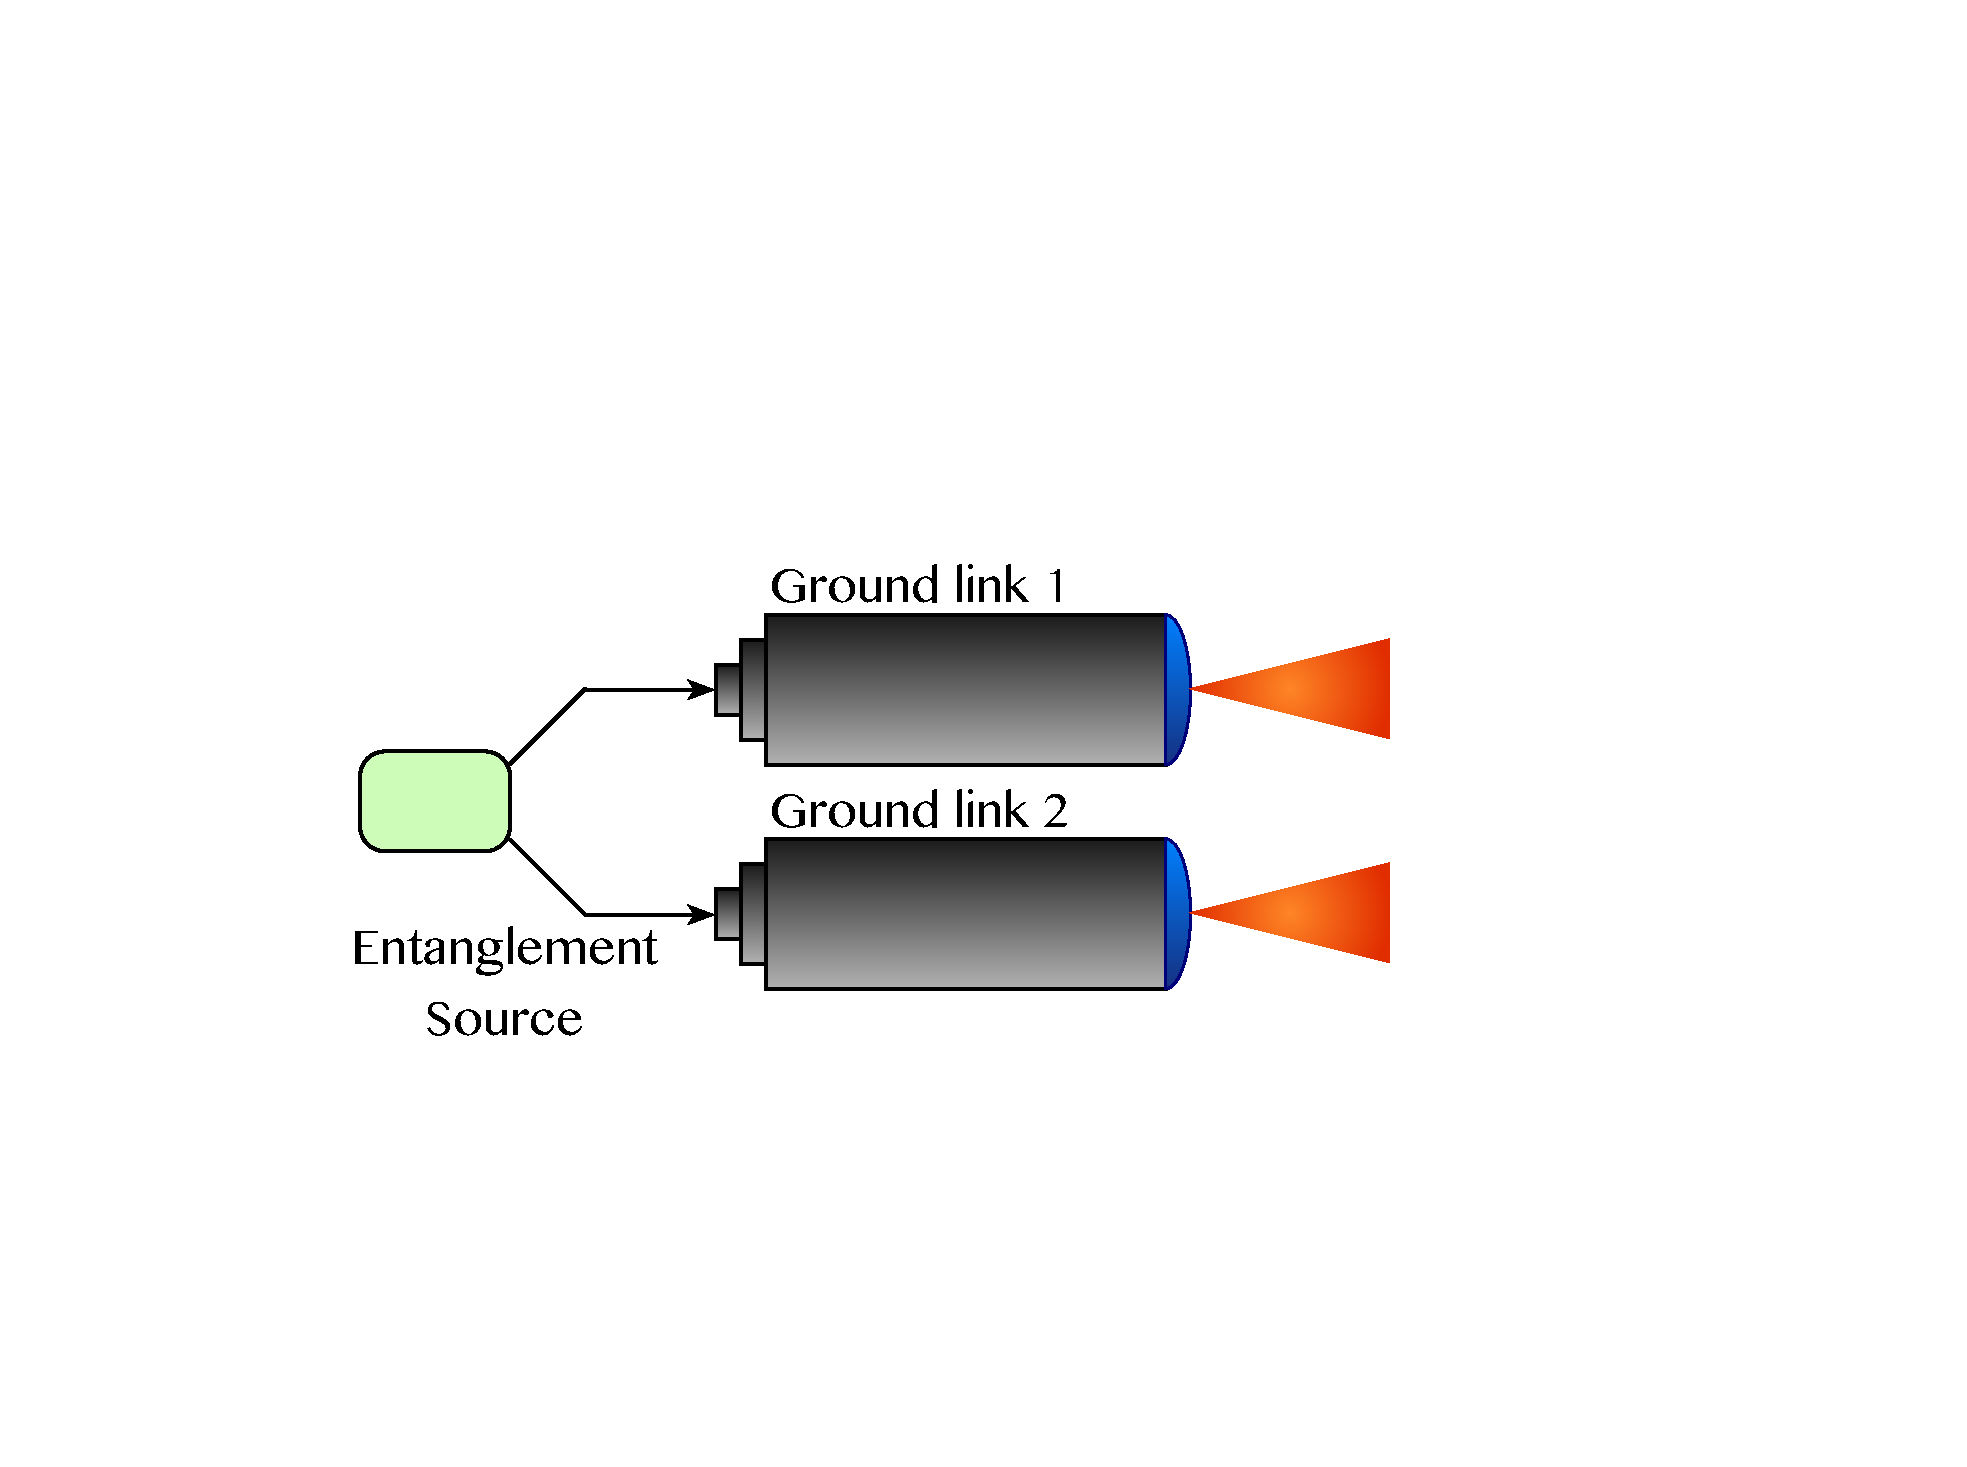
\includegraphics[width=0.47\textwidth]{first_gen_satellite}
\caption{First-generation satellite\index{First-generation quantum satellites} for entanglement distribution. The on-board entanglement source couples to two telescopes, which lock onto independent ground stations using laser tracking\index{Laser tracking}.}\label{fig:first_gen_sat}	
\end{figure}

To facilitate a true global network, next-generation satellites\index{Next-generation quantum satellites} will need to form a constellation\index{Constellation network} sufficiently dense that every point on the Earth's surface is always within line of sight of at least one satellite (Fig.~\ref{fig:sat_honeycomb}).

\begin{figure}[!htb]
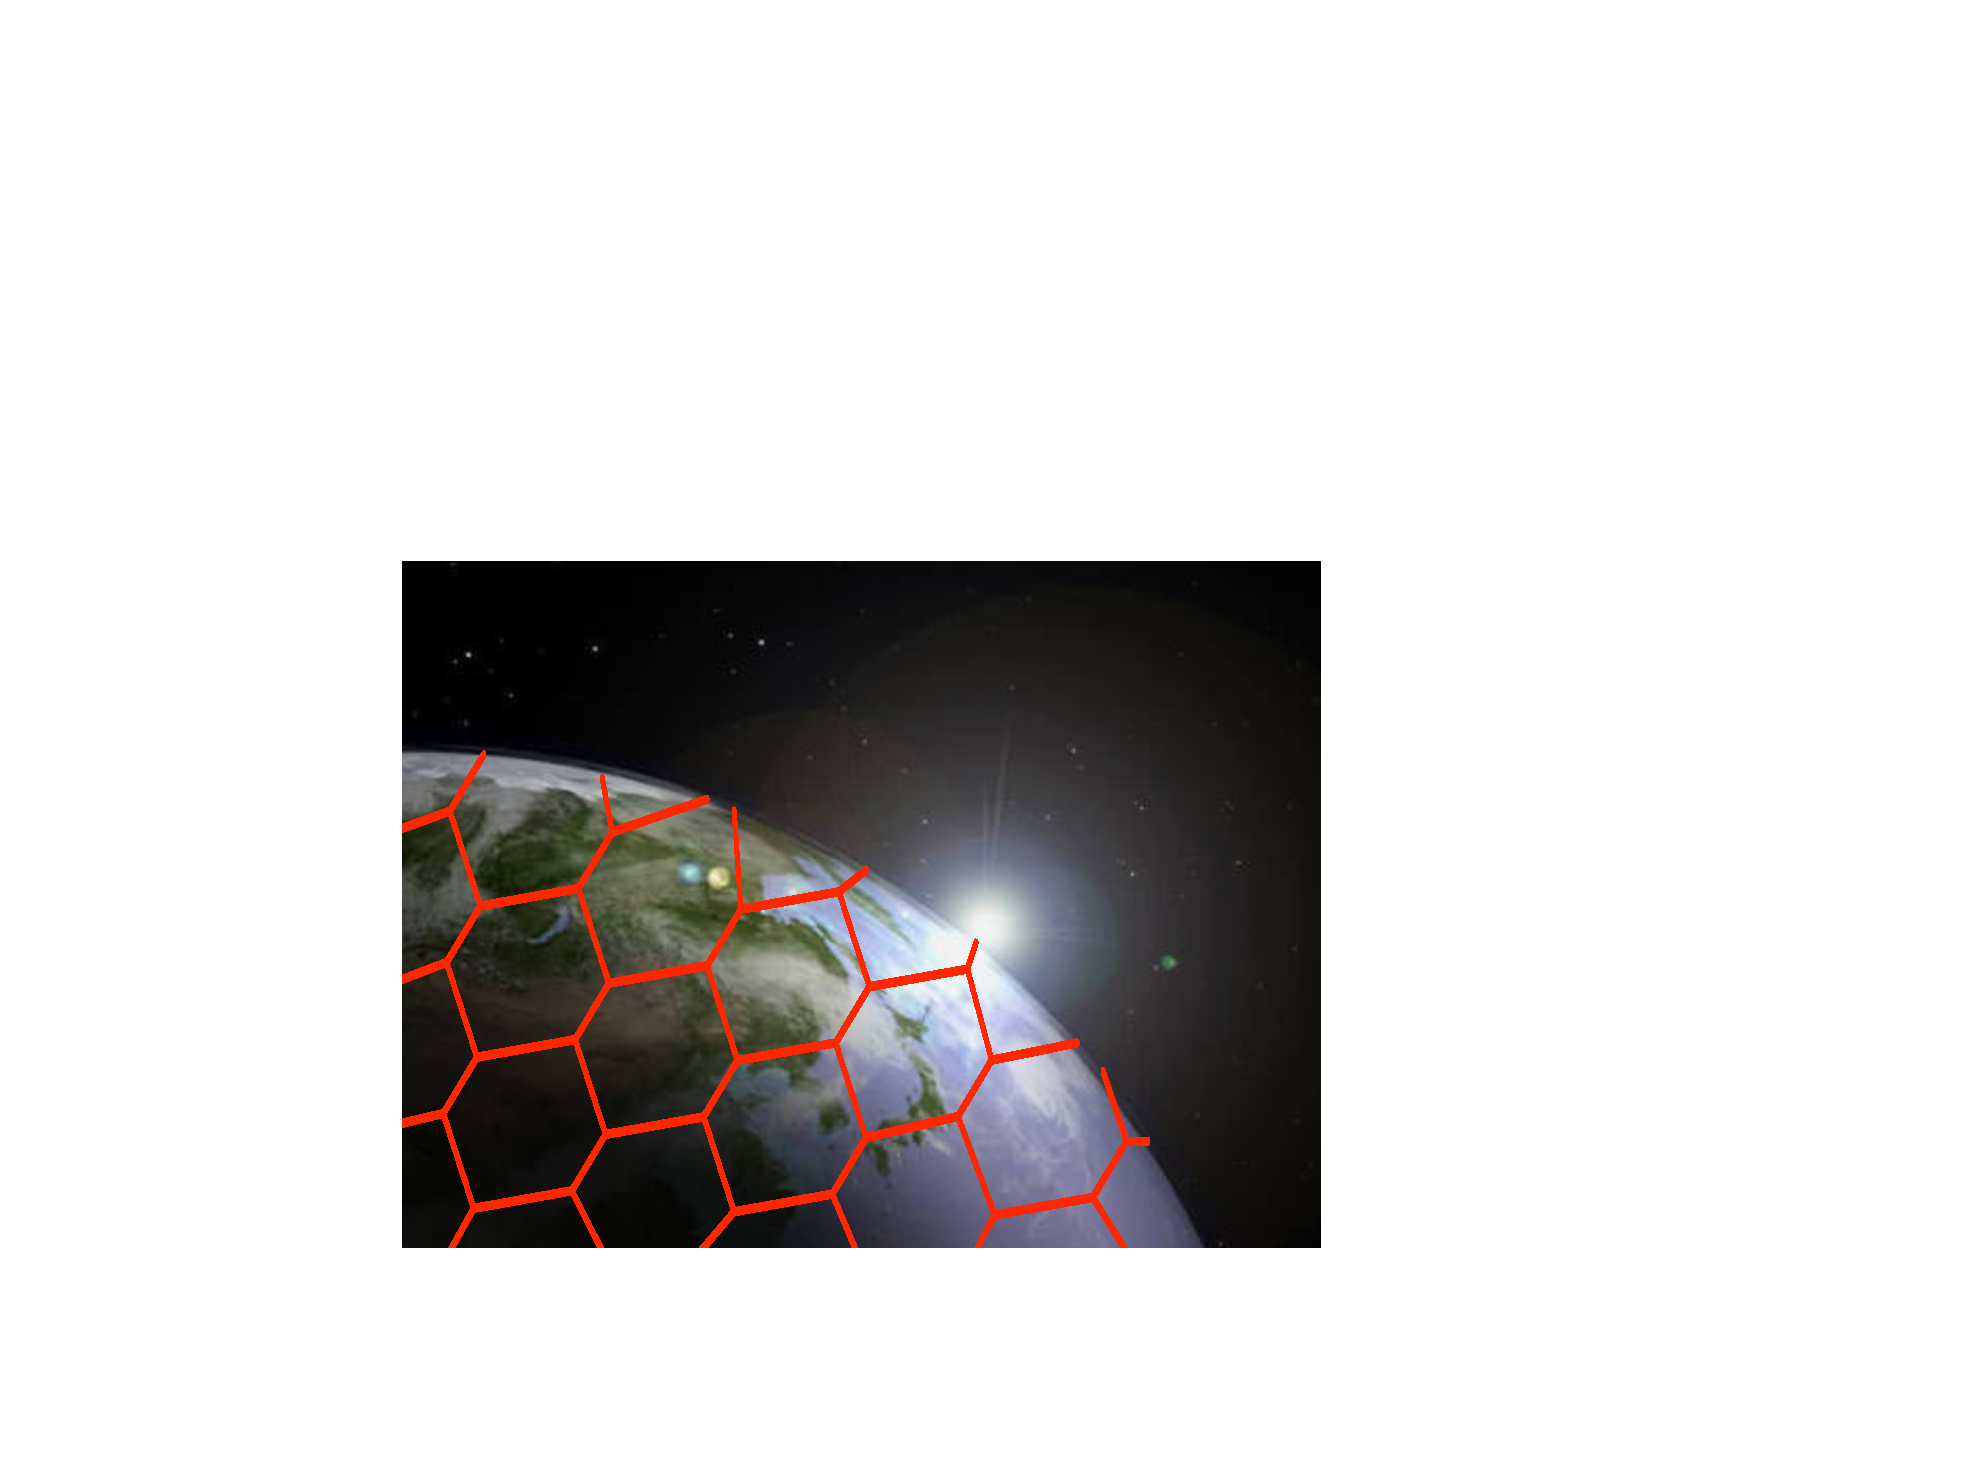
\includegraphics[width=0.47\textwidth]{satellite_honeycomb_lattice}
\caption{A honeycomb lattice\index{Honeycomb lattice} is the lowest order two-dimensional lattice that could be employed to construct a satellite constellation\index{Constellation network} network covering the Earth. Edges represent quantum communications channels, and their intersections are where the satellites reside. Such a network will require next-generation satellites\index{Next-generation satellites} with satellite-to-satellite links.}\label{fig:sat_honeycomb}	
\end{figure}

To enable a constellation, the satellites will need satellite-to-satellite links in addition to the satellite-to-ground links, such that they can relay the entanglement around the curvature of the Earth to overcome line-of-sight limitations. Additionally, they will need to do more than just prepare entangled states, but also perform entangling measurements, such that they can be configured as a quantum repeater network\index{Quantum repeater networks}. A concept model for a next-generation satellite with these essential capabilities is shown in Fig.~\ref{fig:next_gen_sat}.

\begin{figure}[!htb]
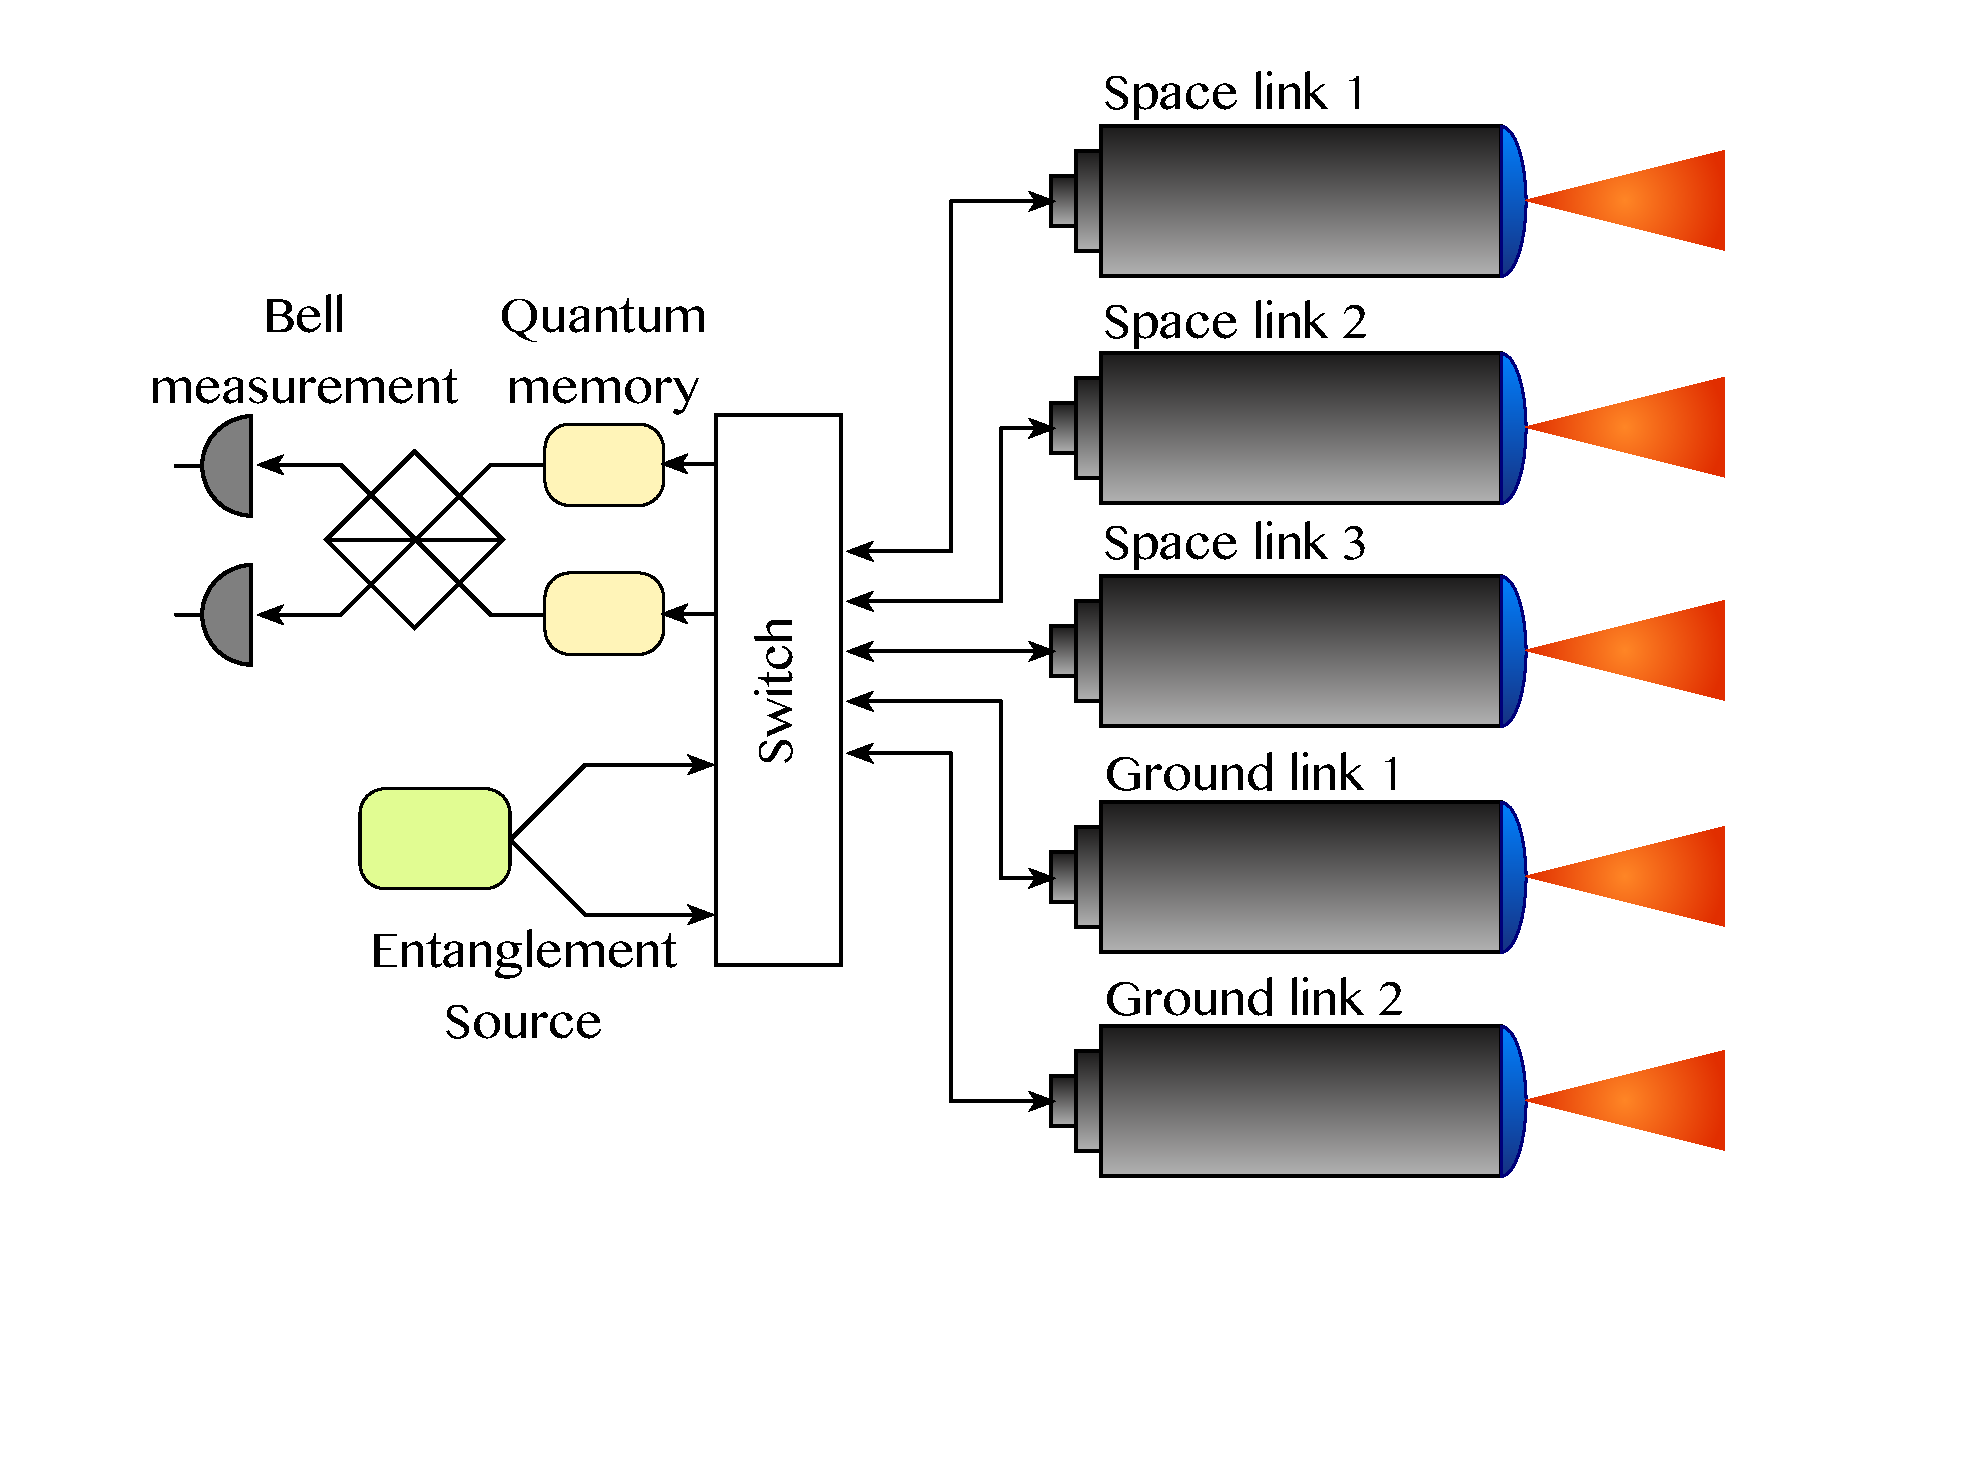
\includegraphics[width=0.47\textwidth]{next_gen_satellite}
\caption{A basic layout for how next-generation quantum satellites might be constructed. Each satellite is capable of both entangled state preparation, as well as entangling measurements. There are three space links for communicating with neighbouring satellites so as to enable a honeycomb lattice configuration, as well as two ground links, as per the first-generation satellite. The switch at the centre must be universal to enable arbitrary pairs of telescopes to couple with either the entanglement source or entangling measurement. The quantum memories\index{Quantum memory} prior to the entangling measurement facilitate synchronising distinct photons with different arrival times such that they can interfere.}\label{fig:next_gen_sat}	
\end{figure}

While the next-generation satellite may appear only incrementally more complex than the first-generation one, it is in fact far more technologically challenging. The main obstacle is that when performing entangling measurements, photons must arrive at the detector simultaneously. Obviously this is hard to enforce in space over long distances on fast-moving objects. Therefore quantum memories\index{Quantum memory} will be required, such that the first of two arriving photons is held in memory until the second one arrives, at which point it is read out from memory and the two photons are jointly measured. Unfortunately, such quantum memories are still very much in their infancy, and not reliable enough or of sufficient quality that they are ready for prime-time applications like a global space-based repeater network. It is unclear how far off these technologies are, despite being under intense investigation.

A global constellation network\index{Constellation network} may require hundreds or thousands of individual satellites. The key to deploying such a network will be via economies of scale\index{Economies of scale}. We must design a single standardised satellite (for example along the lines of that shown in Fig.~\ref{fig:next_gen_sat}), rather than a variety of more specialised models, make it as minimalistic as possible, and then mass produce them on a large scale. With this approach we can hope for economical deployment of a true space-based point-to-point\index{Point-to-point network} global network.

The Chinese have successfully launched and demonstrated the first quantum satellite. This marks the beginning of the quantum space race\index{Space race}. Who will respond? For he who achieves a global network first will wield a huge competitive technological advantage in the upcoming era of the quantum internet and all its foreseeable and unforeseeable applications.

%
% The Quantum Mind
%

\subsection{The quantum mind}\index{Quantum mind}

\comment{To do: quantum machine learning and AI.}

%
% The Quantum Singularity
%

%
% Essay: The Quantum Singularity
%

\section{The quantum singularity} \label{sec:singularity} \index{Quantum singularity}

\dropcap{I}{s} there a point of no return for the quantum internet? We argue there is, which we refer to as the \textit{quantum singularity}, characterised by the forthcoming qualities.

\latinquote{Adiuva nos Deus.}

%
% Economic No Return
%

\subsection{Economic no return}\index{Economic no return}

Since there is positive computational leverage associated with quantum networking -- to \textit{all} participating parties, irrespective of size -- this creates a self-reinforcing economic quantum ecosystem, whereby all market participants are increasingly incentivised to continue contributing to the network, exponentially enhancing its collective power, with ever increasing returns over time for all. We will have reached a point of self-reinforcing exponential growth, driven by market forces. Because of the exponential scaling in computational power, it only becomes rational to ever-increasingly invest into further expansion, as every new qubit enhances the network more than the last.

%
% Self-Improvement
%

\subsection{Self-improvement}\index{Self-improvement}

Since quantum algorithms provide quadratic speedup to \textbf{NP}-complete problems, and hence many optimisation problems, it follows that the existing distributed quantum computer will be able to perform self-enhancement by improving network routing efficiency, resource allocation, and even the design of the next generation of quantum computers, compared to what could be achieved using classical scheduling and optimisation algorithms.

This self-improvement will also be self-reinforcing -- as the quantum network becomes more powerful, its capacity for self-improvement will accelerate, at which point the self-enhancement becomes self-sustaining, without the need for human intervention or classical computers to guide the way.

%
% Intellectual No Return
%

\subsection{Intellectual no return}\index{Intellectual no return}

With the ability to perform accelerated machine learning, with post-classical capability, we will inevitably reach a point at which the quantum network becomes more intelligent than mankind collectively. It will be able to invent, discover, prove, learn, and plan exponentially better than the human race who built it. At this point in time the entire economic framework for humanity will need to be reevaluated.

How can there be economic demand for human labour when our technology makes both manual and intellectual human capital redundant? Conventional mechanical machines can already largely automate manual labour, making many occupations from our parents' generation obsolete. If next the quantum network makes human intellect redundant, what will the place for the human race be in the world? Can a capitalist economic model survive the collapse in demand for human labour? How can money circulate in its absence? What paradigm will emerge in its place?

\comment{Review}